\subsection{LowProFool}
\subsubsection{概要}
表形式データに対する敵対的サンプルの生成手法として,Balletらが提案したLowProFool\cite{ballet2019imperceptible}がある.表形式データの特徴として識別に寄与する各特徴量の重要度が異なることが多い.LowProFoolはこの点に着目し各特徴量の重要度を元データから算出し,それに基づいたノイズを付加することで誤分類を引き起こし,検知されにくい敵対的サンプルを生成する.この手法は,深層学習モデルを用いて敵対的サンプルを用いて敵対的サンプルを生成する点に特徴がある.具体的には,ニューラルネットワークを用いて元データに対するノイズを最適化し,モデルの誤分類を誘発する.このアプローチにより,より高度な特徴抽出とノイズ付加が可能となり,従来の手法よりも効果的な敵対的サンプルを生成することができる.

\subsubsection{LowProFoolの問題設定}
LowProFoolは検知されにくい敵対的サンプルを生成するため,以下の最適化問題を解く.
\autoequation{\bm{r}^* = \mathrm{arg}_{\bm{r}} \min d(\bm{r}) \text{ for } \bm{r} \in \mathbb{R}^D}
\autoequation{\mathrm{s.t. }  f(\bm{x}) = s \neq f(\bm{x}+\bm{r}^*) = t,  \bm{x}+\bm{r}^* \in A}

ここで,$d(\bm{r})$ はノイズの大きさを評価する指標であり,以下のように定義される.
\autoequation{d_{\bm{v}}(r) = ||\bm{r} \odot \bm{v}||^2_p}

式(2)における $\bm{v}$ は各特徴量の重要度を表すベクトルであり, $\bm{r}$ はノイズベクトルである. $\odot$ はアダマール積を表し,各特徴量ごとに特徴量とノイズの掛け算を行っている. $||\odot||^2_p$ は $\ell_2$ ノルムを表す.また,ノイズベクトル $\bm{r}$ は元データの特徴量数と同じ $D$ 次元の実数空間から選ばれる.これにより,重要度が高い特徴量には小さなノイズが適用され,重要度が低い特徴量には比較的大きなノイズが許容される.

式(3)の一つ目の制約 $f(\bm{x}) = s \neq f(\bm{x}+\bm{r}^*) = t$ は,元データ $\bm{x}$ の分類結果 $s$ とノイズを付加したデータ $\bm{x}+\bm{r}^*$ の分類結果 $t$ が異なることを要求する.二つ目の制約 $\bm{x}+\bm{r}^* \in A$ は,生成された敵対的サンプルが現実的な値域 $A$ に収まることを保証する.$A$ は,元データから各特徴量に対する最小値から最大値の集合であり,元データの分布を大きく崩さないようにするために用いられる.

% 目的関数について
LowProFoolでは上記の最適化問題を解くため,以下の目的関数 $g(\bm{r})$ を使用する.これを式(5)を定義する.

\autoequation{g(r) = L(\bm{x}+\bm{r}, t) + \lambda ||\bm{v} \odot \bm{r}||_2}

ここで, $L(\bm{x}+\bm{r}, t)$ は損失関数であり, $\bm{x}+\bm{r}$ がラベル $t$ に分類されるようにするための誤差を表す. $\lambda$ は正則化パラメータであり,ノイズの大きさを制御するために使用される.
これにより,元データの特徴量の重要度を考慮しつつ,検出されにくい敵対的サンプル $\bm{x}'$ を生成する.

\subsubsection{LowProFoolのアルゴリズム}
次にLowProFoolのアルゴリズムを示す.アルゴリズムの各ステップは以下の通りである.
\begin{algorithm_step}
    \item[Step 1)] アルゴリズムで使用する変数の初期化を行う.ノイズベクトル $\bm{r}$ を
        ゼロベクトルで初期化する.また,初期サンプル $\bm{x}_0$ を元のサンプル $\bm{x}$ とする.
    
    \item[Step 2)] 最大反復回数 $N$ まで以下の計算を繰り返す.まず,前述の目的関数 
        $g(r) = L(\bm{x}+\bm{r}, t) + \lambda ||\bm{v} \odot \bm{r}||_2$ の勾配を計算する.
        次に,計算された勾配に基づいてノイズベクトル $\bm{r}$ を更新する.
        更新されたサンプルが有効な値域に収まるようクリッピングを行う.
    
    \item[Step 3)] 最適な敵対的サンプルの選択を行う.生成された敵対的サンプルの中から,
        元のサンプルとは異なるクラスに分類される($f(\bm{x}_i) \neq f(\bm{x}_0)$)ことと,
        検知されにくさの指標 $d_v(\bm{x}_i)$ が最小となるものを選ぶ.
    
    \item[Step 4)] 選択された敵対的サンプル $\bm{x}'$ を返す.
    \end{algorithm_step}


このアルゴリズムの特徴は,各反復において特徴量の重要度を考慮しながらノイズを更新する点にある.重要度の高い特徴量に対しては小さな摂動に抑えられ,重要度の低い特徴量により大きな摂動が許容される.これにより,分類結果を変更しつつも,検知されにくい敵対的サンプルの生成が可能となる.
また,クリッピング操作により,生成されるサンプルが常に有効な値域に収まることが保証される.例えば,年齢のような非負の特徴量が負の値を取ることを防ぐことができる.


\subsection{特徴量の重要度算出方法}

前述の通り,識別に寄与する特徴量を考慮した上で,ノイズを付加する.特徴量重要度 $\bm{v}$ の算出は,分類結果に対する各特徴量の相関係数を用いることが提案されていた.ピアソンの相関係数を用いて以下のように定義される.

\autoequation{v_i = \cfrac{|\rho_{\bm{X_i},Y}|}{\|\rho_{\bm{X_i},Y}\|^2_2}}
$\|\rho_{\bm{X_i},Y}\|$ は $i$ 番目の特徴量 $\bm{X_i}$ と目的変数 $\bm{Y}$ の相関係数を示している.各特徴量と目的変数の関係性の強さを示す指標であり,値が大きいほどその特徴量が分類結果に寄与していることを意味する.また,分母は全ての特徴量の寄与度の二乗和の平方根を表し,全体の相関のスケールに対して分子を正規化している.これにより,$d$ 個の特徴量についてまとめた特徴量重要度 $[ \bm{v} = \{v_1, v_2, \cdots, v_d\} ]$ は,各特徴量が持つ相関の相対的な重要性を反映した値となる.この特性により,上記のアルゴリズムでは最小化を行うため,相関係数が大きい特徴量に対しては小さなノイズが付加されることになり,重要度を表現することができる.

% \begin{figure}[H]
%     \centering
%     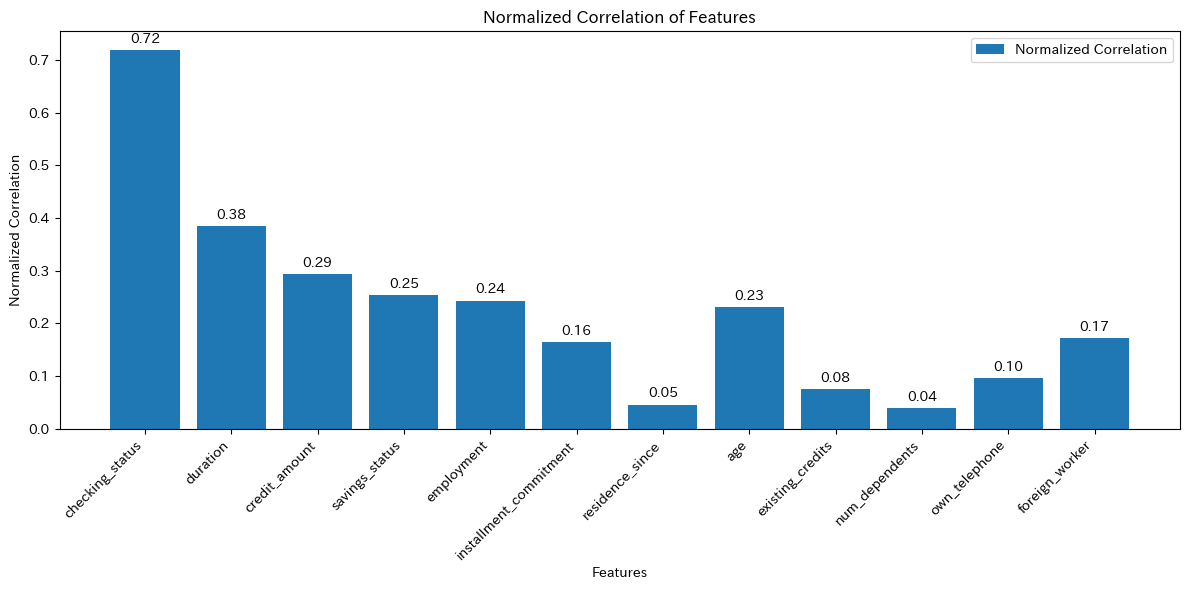
\includegraphics[width=0.8\textwidth]{images/従来手法_特徴量重要度.png}
%     \caption{従来手法:各特徴量における重要度}
%     \label{fig:default_method_feature_importance}
% \end{figure}


\subsection{従来手法の課題}

この手法について二つの問題をはらんでいる可能性がある

一つ目に特定の特徴量に対するノイズが集中してしまう可能性があることである.特徴量重要度の算出方法(式(6))において,相関係数に対して正規化処理を行っている.機械学習手法を利用する際に,特徴量ごとにとり得る範囲(スケール)が大きく異なることで過学習などの問題が発生してしまう可能性がある.正規化はこの問題を抑えるための手法として有用である.\cite{LawOfAwesomeDataScientist}相関係数の絶対値では $0~1$ の範囲で特徴量の性質を表している.追加で正規化を行うと繊細な重要度を表現が難しくなる.特に重要度が極端に大きい特徴量に対してノイズを大きく避けるため,次に重要な特徴量へのノイズ集中してしまっている可能性をはらんでいる.よって元データの特徴を捉えた特徴量重要度の算出が重要になっている.

二つ目に,敵対的サンプルの出力が連続値であることが挙げられる.離散値を持つ特徴量に対して連続値を取ることで,現実的でない値をとってしまっている.このため,連続値の敵対的サンプルを離散値に変換する必要がある.

これらの課題に対して,次節では改良手法を提案する.